\begin{table}[!ht]
    \centering
    \resizebox{\columnwidth}{!}{\begin{tabular}{|c|c|c|c|} 
    \hline
    Component & P & Q & Requirement \\
    \hline
    Calcium & 12 units & 3 units & $\geq 240$ units \\ 
    \hline
    Iron & 4 units & 20 units & $\geq 460$ units \\ 
    \hline
    Cholesterol & 6 units & 4 units & $\leq 300$ units\\ 
    \hline
    Vitamin A & 6 units & 3 units & \\ 
    \hline
    \end{tabular}}
    \caption{Diet Requirements}
    \label{opt/36/tab:table1}
    \end{table}
    Let the number of packets of food P be $x$ and the number of packets of food Q be $y$  such that 
    \begin{align}
        x \geq 0 \\
        y \geq 0 
    \end{align}
    According to the question,
    \begin{align}
        12x+3y &\geq 240 \\
        \implies -4x-y &\leq -80 \\
    \end{align}
    and,
    \begin{align}
        4x+20y &\geq 460 \\
        \implies -x-5y &\leq -115 
    \end{align}
    and,
    \begin{align}
         6x+4y &\leq 300 \\
        \implies 3x+2y &\leq 150 
    \end{align}
    $\therefore$ Our problem is
    \begin{align}
            \min_{\vec{x}} Z &= \myvec{6 & 3}\vec{x}\\
            s.t. \quad 
            \myvec{-4 & -1 \\ -1 & -5 \\ 3 & 2 }\vec{x} &\preceq \myvec{-80\\-115\\150} \\
            \vec{-x} &\preceq \vec{0}
    \end{align}
    Lagrangian function is given by
    \begin{equation}
    \begin{aligned}
        &L(\vec{x},\boldsymbol{\lambda}) \\ &= \myvec{6 & 3}\vec{x}+\lcbrak{\sbrak{\myvec{-4 & -1}\vec{x}+80}} \\ &+ \sbrak{\myvec{-1 & -5}\vec{x}+115} +\sbrak{\myvec{3 & 2}\vec{x}-150} \\ &+ \sbrak{\myvec{-1 & 0}\vec{x}} +\rcbrak{\sbrak{\myvec{0 & -1}\vec{x}}}\boldsymbol{\lambda}
    \end{aligned}
    \end{equation}
    where,
    \begin{align}
        \boldsymbol{\lambda} &= \myvec{\lambda_1 \\ \lambda_2 \\ \lambda_3 \\ \lambda_4 \\ \lambda_5 \\ \lambda_6}
    \end{align}
    Now,
    \begin{align}
        \nabla L(\vec{x},\boldsymbol{\lambda}) &= \myvec{6+ \myvec{-4 & -1 & 3 & -1 & 0 }\boldsymbol{\lambda}\\ 3+\myvec{-1 & -5 & 2 & 0 & -1}\boldsymbol{\lambda} \\ \myvec{-4 & -1}\vec{x}+80 \\ \myvec{-1 & -5}\vec{x}+115 \\ \myvec{3 & 2}\vec{x}-150 \\ \myvec{-1 & 0}\vec{x} \\ \myvec{0 & -1}\vec{x}}
    \end{align}
    $\therefore$ Lagrangian matrix is given by
    \begin{align}
        \myvec{0 & 0 & -4 & -1 & 3 & -1 & 0 \\ 0 & 0 & -1 & -5 & 2 & 0 & -1 \\ -4 & -1 & 0 & 0 & 0 & 0 & 0 \\ -1 & -5 & 0 & 0 & 0 & 0 & 0 \\ 3 & 2 & 0 & 0 & 0 & 0 & 0 \\ -1 & 0 & 0 & 0 & 0 & 0 & 0 \\ 0 & -1 & 0 & 0 & 0 & 0 & 0 }\myvec{\vec{x} \\ \boldsymbol{\lambda} } &= \myvec{-6 \\ -3 \\ -80 \\ -115 \\ 150 \\ 0 \\0 }
    \end{align}
    Considering $\lambda_1,\lambda_2$ as only active multiplier,
    \begin{align}
        \myvec{0 & 0 & -4 & -1 \\ 0 & 0 & -1 & -5 \\ -4 & -1 & 0 & 0 \\ -1 & -5 & 0 & 0}\myvec{\vec{x}\\ \boldsymbol{\lambda}} &= \myvec{-6 \\ -3 \\ -80 \\ -115}
    \end{align}
    resulting in,
    \begin{align}
        \myvec{\vec{x} \\ \boldsymbol{\lambda}} &= \myvec{0 & 0 & -4 & -1 \\ 0 & 0 & -1 & -5 \\ -4 & -1 & 0 & 0 \\ -1 & -5 & 0 & 0}^{-1}\myvec{-6 \\ -3 \\ -80 \\ -115}
        \\
        \implies   \myvec{\vec{x} \\ \boldsymbol{\lambda}} &= \myvec{0 & 0 & \frac{-5}{19} & \frac{1}{19} \\ 0 & 0 & \frac{1}{19} & \frac{-4}{19} \\ \frac{-5}{19} & \frac{1}{19} & 0 & 0 \\ \frac{1}{19} & \frac{-4}{19} & 0 & 0}\myvec{-6 \\ -3 \\ -80 \\ -115}
        \\
        \implies \myvec{\vec{x} \\ \boldsymbol{\lambda}} &= \myvec{15 \\ 20 \\ \frac{27}{19} \\ \frac{6}{19} }
    \end{align}
    $\because \boldsymbol{\lambda}=\myvec{\frac{27}{19} \\ \frac{6}{19}} \succ \vec{0} $
    \\
    $\therefore$ Optimal solution is given by
    \begin{align}
        \vec{x} &= \myvec{15\\20} \\
        Z &= \myvec{6 & 3}\vec{x} \\
        &= \myvec{6 & 3}\myvec{15 \\ 20} \\
        &= 150
    \end{align}
    By using cvxpy in python ,
    \begin{align}
        \vec{x}=\myvec{14.99999999\\20.00000001}\\
        Z = 150.00000001
    \end{align}
    Hence ,\boxed{x=15} packets of food P and \boxed{y=20} packets of food Q should be used to minimise the amount of vitamin A in the diet and the minimum amount of vitamin A is \boxed{Z=150} units.  This is verified in Fig. \ref{opt/36/fig:diet problem}	
    %
    \begin{figure}[!ht]
    \centering
    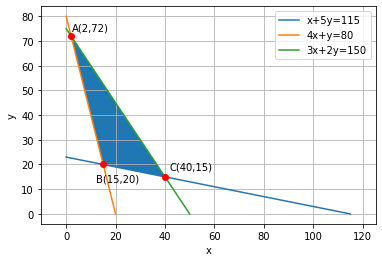
\includegraphics[width=\columnwidth]{solutions/su2021/2/36/Figure12.png}
    \caption{Diet Problem}
    \label{opt/36/fig:diet problem}	
    \end{figure}